\documentclass[12pt]{article}
\usepackage[czech]{babel}
\usepackage[utf8]{inputenc}
\usepackage[plainpages=false,pdfpagelabels,unicode]{hyperref}
\usepackage[pdftex]{graphicx}
\usepackage[margin=2cm, includefoot]{geometry}
\usepackage[version=3]{mhchem}

\begin{document}

\title{Praktikum z fyziky plazmatu \\
Elektrické charakteristiky zapálení diafragmového výboje a generace peroxidu vodíku diafragmovým výbojem ve vodných roztocích}
\author{Vlasta Štěpánová a Pavel Ondračka}
\maketitle

\section{Teorie}

\subsection{Elektrický výboj v kapalině}
V tomto praktiku byl zkoumán diafragmový výboj, jenž vzniká mezi dvěmi plochými elektrodami ponořenými v kapalině oddělenými dielektrickou překážkou s malým otvorem -- diafragmou. Výboj je iniciován aplikací
konstantního stejnosměrného napětí. Intenzita elektrického pole mezi elektrodami ale není
konstantní, výrazně roste v oblasti otvoru v diafragmě. Zde dosahuje velmi vysokých hodnot
($>$ $10^5$ Vm$^{-1}$), a proto dochází v těchto místech k elektrickému průrazu -- vzniku plazmatu
(výboje). 

Princip vzniku výboje spočívá v tom, že průchodem elektrického proudu se roztok v reaktoru zahřívá, a to
především v oblasti otvoru v diafragmě. Zde je nejvyšší proudová hustota a proto se uvolňují bubliny páry. Při dostatečně vysokém gradientu napětí dojde k průrazu primárně v těchto bublinách. Výboj se pak dále šíří formou plazmových kanálů roztokem.

Významným rysem generace stejnosměrného diafragmového výboje je tvorba dvou typů plaz\-mo\-vých kanálů na každé
straně diafragmy. Na straně kladně nabité elektrody jsou tvořeny záporné plazmové kanály
(„streamery“), které zaujímají hustou síť tenkých kanálů vyplňujících polokulový prostor.
Naopak na straně záporné elektrody jsou tvořeny kladné „streamery“ obsahující jen jeden
nebo několik rozvětvených kanálů. Rychlost jejich šíření je vyšší než u záporných
„streamerů“. Experimentální aparaturu tvořil reaktor o objemu 3,5\,l rozdělený diafragmou na anodovou a katodovou část. Diafragma byla destička vyrobená z polyethylentereftalátu o tloušťce 0,5\,mm a s otvorem o průměru 0,4\,mm. Měření napětí a proudu bylo prováděno dvoukanálovým osciloskopem. Na jednom kanálu bylo měřeno napětí na zdroji, na druhém napětí na známém odporu (5,13\,$\Omega$), z něj byl poté vypočítán proud. Schéma použité aparatury je na obrázku \ref{schema}.

\subsection{Generace peroxidu vodíku}
V plazmatu dochází k tvorbě různých reaktivních chemických částic. Mezi ně patří radikály ·OH, ·H, ·O, ·HO$_2$), neutrální molekuly (\ce{H2O2}, \ce{H2},
\ce{O2}) a ionty (\ce{O2^-}). Za nejdůležitější z těchto částic jsou považovány hydroxylové a kyslíkové
radikály (·OH, ·O), ozón (\ce{O3}) a peroxid vodíku (\ce{H2O2}), které se významně podílejí na
oxidačních procesech probíhajících v kapalné fázi během výboje.

Mechanismy tvorby ·OH a ·H radikálů elektrickým výbojem v kapalné fázi:
$$
\mathrm{disociace:\,\,\,} \ce{H2O + e- -> OH. + H. + e-}\,\,\,\,\,\,
$$ $$
\mathrm{ionizace:\,\,\,} \ce{ H2O + e- -> H2O+. + 2e-}\,\,\,\,\,\,\,\,\,\,\,\,\,\,
$$ $$
\mathrm{disociace:\,\,\, } \ce{ H2O+. + H2O -> H3O+ + OH.}
$$ $$
\mathrm{tvorba\,peroxidu\,vodiku:\,\,\,} \ce{2OH. -> H2O2} \,\,\,\,\,\,\, 
$$

V závislosti na parametrech výboje se mění poměr mezi výše uvedenými reakcemi a tak radikály mohou buď reagovat navzájem a vytvářet tak
výsledné molekuly \ce{H2} a \ce{H2O2}, nebo znovu vytvářet vodu, anebo difundovat od sebe a být
dostupné pro další reakce v roztoku.

Systém lze považovat za sled dvou oddělených reakcí probíhajících současně:
$$
\ce{H2O -> OH. + H.}
$$ $$
\ce{2H2O -> H2O2 + H2}
$$
Tyto dvě rovnice jsou považovány za hlavní reakce iniciované elektrickým výbojem
ve vodě, $k_{\ce{OH}}$ a $k_{\ce{H2O2}}$ jsou jejich rychlostní konstanty. Jelikož koncentrace vody zůstává
přibližně konstantní, reakce jsou považovány za reakce nultého řádu. Z toho vyplývá, že koncentrace OH radikálů i peroxidu vodíku v čase narůstá lineárně.

Pro určení koncentrace \ce{H2O2} používáme titanové činidlo, jehož reakci s \ce{H2O2} lze popsat rovnicí \ce{Ti^{4+} + H2O2 + 2H2O -> TiO2.H2O2 + 4H+}. Výsledný komplex kyseliny peroxotitaničité způsobuje výrazné žluté zbarvení a měřením absorpce na spektrofotometru lze určit koncentraci \ce{H2O2} v roztoku. 





\begin{figure}[htbp]
\begin{center}
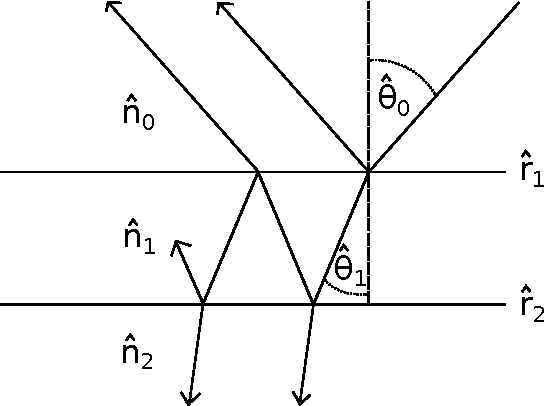
\includegraphics[width=12cm]{schema.pdf}
\caption{Schéma aparatury, A -- anoda, K -- katoda, D -- diafragma, O -- osciloskop (na kanálu 1 je vysokonapěťová sonda)}
\label{schema}
\end{center}
\end{figure}

\section{Měření}
Aparatura byla naplněna solným roztokem (0,9\,g NaCl v 3,5\,l) a byla naměřena vodivost roztoku -- 302\,mS/cm. Poté byla naměřena VA charakteristika výboje a to jak při zvyšování napětí tak i při následném snižování, to je na obrázku \ref{VA}. Zápalné napětí je přibližně 1200\,V, bylo určeno jako bod kde dochází na VA charakteristice ke zlomu. Napětí nebylo úplně konstantní, ale, kvůli nízké kvalitě zdroje, mírně kmitalo s frekvencí 50\,Hz, jeho střední hodnota byla určena osciloskopem (s vysokonapěťovou sondou pro měření vysokého napětí na kanálu 1). Průběhy časového vývoje napětí a proudu jsou na obrázcích \ref{vyvoj1}, \ref{vyvoj2} a \ref{vyvoj3}.  Následně byl roztok vylit, udělán nový, tentokrát s naměřenou vodivostí 296\,mS/cm, a byl zapálen výboj s konstantními hodnotami středního napětí a proudu: 1120\,V a 0,18\,A. V pravidelných intervalech dvou minut byly z anodové i katodové části aparatury odebírány vzorky roztoku, do kterých bylo následně přidáno titanové činidlo, které reaguje s peroxidem vodíku za vzniku žlutého barviva. Na spektrofotometru byla poté, dle míry zbarvení, určena koncentrace peroxidu vodíku v jednotlivých vzorcích. Z fitu časového vývoje koncentrace (obrázek \ref{koncentrace}) byla určena rychlostní konstanta $k_{\ce{H2O2}}$ pro anodovou i katodovou část aparatury, ta je pro katodovou část (1,70$\pm$0,11)·10$^{-2}$ mmol·l$^{-1}$·s$^{-1}$ a pro anodovou (4,17$\pm$1,6)·10$^{-2}$ mmol·l$^{-1}$·s$^{-1}$. Hodnoty vodivosti po skončení výboje nebyly již z časových důvodů měřeny.

\begin{figure}[htbp]
\begin{center}
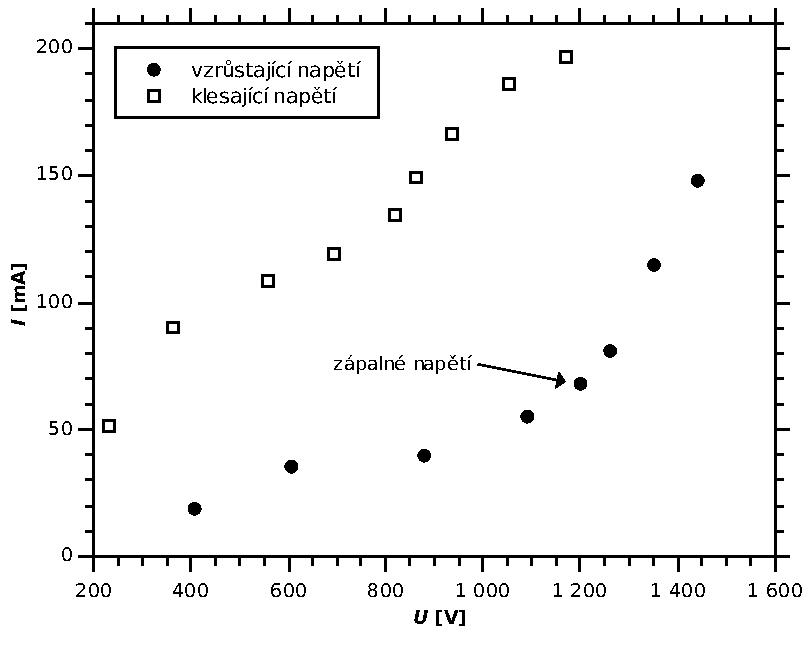
\includegraphics[width=12cm]{Graph1.pdf}
\caption{VA charakteristika diafragmového výboje s přibližnou hodnotou zápalného napětí}
\label{VA}
\end{center}
\end{figure}

\begin{figure}[htbp]
\begin{center}
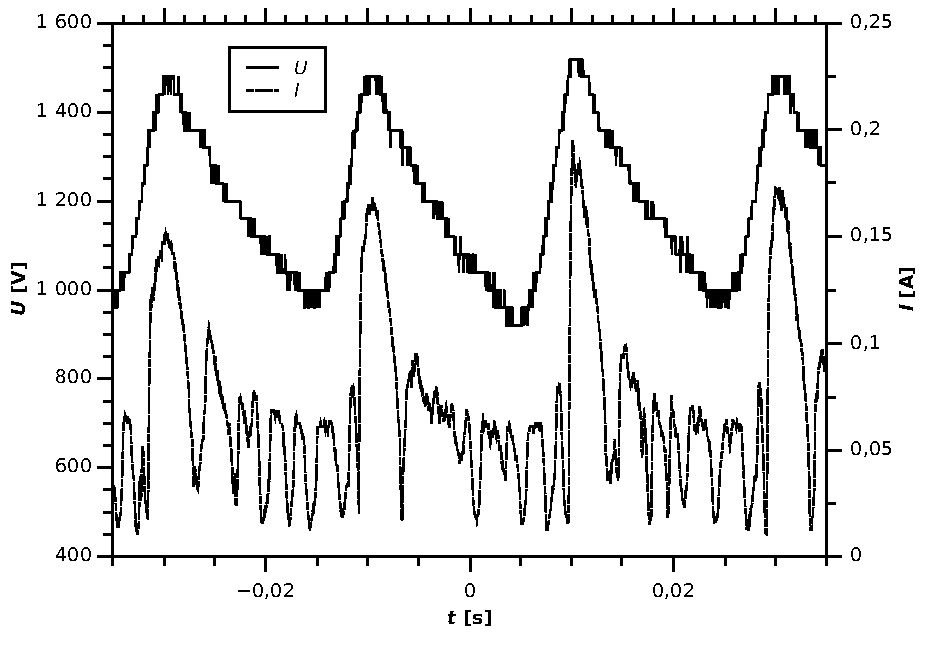
\includegraphics[width=12cm]{zapalnenapeti.pdf}
\caption{Časový průběh napětí a proudu v bodě zápalného napětí}
\label{vyvoj1}
\end{center}
\end{figure}

\begin{figure}[htbp]
\begin{center}
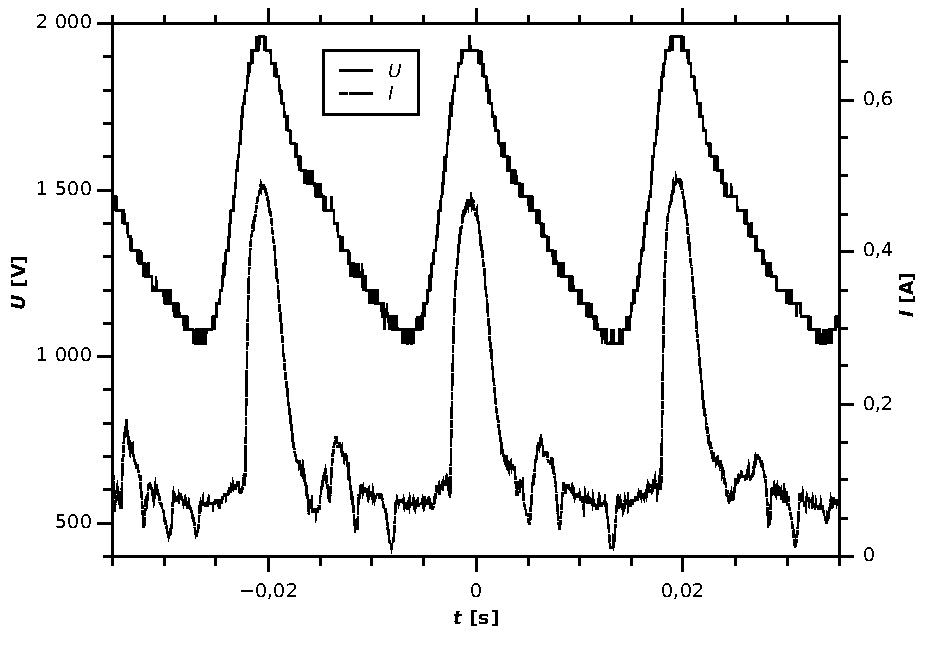
\includegraphics[width=12cm]{horicivyboj.pdf}
\caption{Časový průběh napětí a proudu v bodě kde již hoří výboj (střední napětí 1440\,V)}
\label{vyvoj2}
\end{center}
\end{figure}

\begin{figure}[htbp]
\begin{center}
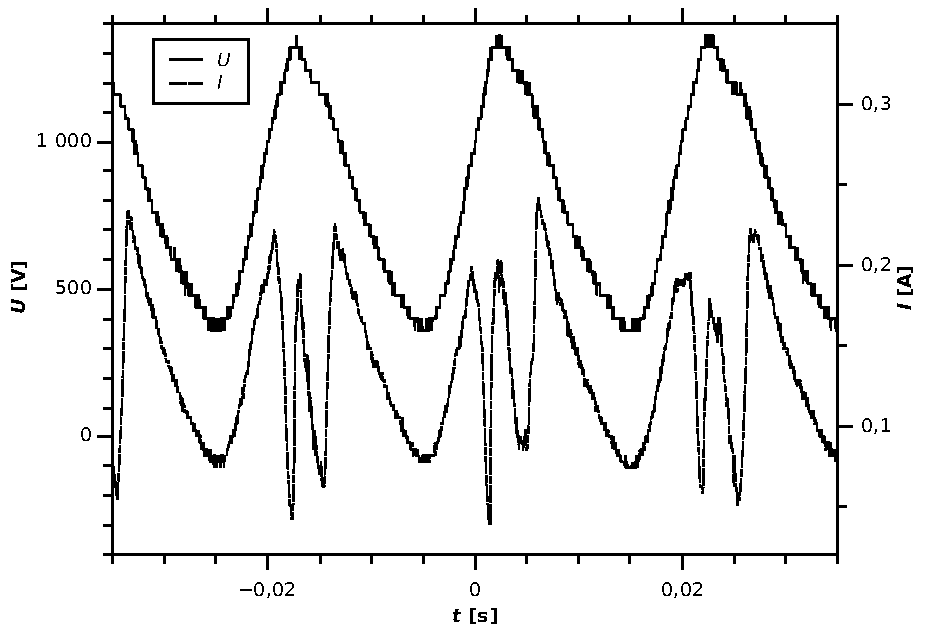
\includegraphics[width=12cm]{klesajicinapeti.pdf}
\caption{Časový průběh napětí a proudu při při snižování napětí (střední napětí 816\,V)}
\label{vyvoj3}
\end{center}
\end{figure}

\begin{figure}[htbp]
\begin{center}
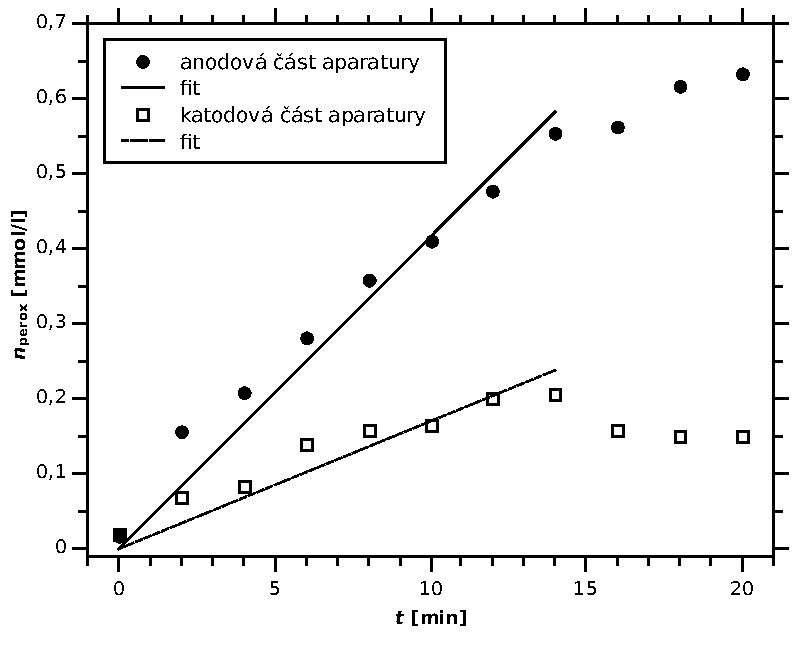
\includegraphics[width=12cm]{Graph2.pdf}
\caption{Časový vývoj koncentrace peroxidu vodíku v aparatuře}
\label{koncentrace}
\end{center}
\end{figure}

\newpage

\section{Závěr}
Měření proběhlo úspěšně. Podařilo se nám úspěšně zapálit diafragmový výboj a naměřit jeho VA charakteristiku. Pro nízké napětí proud roste přibližně lineárně až v bodě zápalného napětí dochází ke vzniku bublinek a zapálení výboje, čemuž odpovídá prudký nárůst proudu. Při snižování napětí vykazuje VA jednak zvýšení napětí při úbytku proudu a také hysterezi, to bylo pravděpodobně způsobeno tím, že mezi posledním vzestupným a prvním sestupným měřením uplynul delší časový úsek během kterého stále hořel výboj a došlo k vypálení velké díry do~diafragmy, zvětšení koncentrace nabitých části a také změně vodivosti roztoku (která bohužel nebyla na konci experimentu změřena). Při měření časového vývoje koncentrace peroxidu vodíku se ukázalo, že ze začátku roste koncentrace lineárně, při delších časech se nárůst zpomalí, toto si vysvětluji tím, že při vyšších koncentracích peroxidu vodíku se zvětšuje pravděpodobnost následných reakcí. Navíc měření bylo prováděno s přerušeními, protože bylo pokaždé potřeba vypnout výboj kvůli odběru vzorků, což se mohlo na grafu také projevit. Pokles koncentrace v katodové části aparatury pro větší časy je téměř jistě experimentální chyba, která se dá teoreticky jen těžko vysvětlit. Také se podařilo potvrdit rozdílný charakter výboje v anodové a katodové části aparatury, který se projevil rozdílnou koncentrací \ce{H2O2} v obou částech.

\end{document}
